\documentclass{beamer}

\usepackage[french]{babel}
\usepackage[utf8]{inputenc}

\usepackage[T1]{fontenc}

\usepackage{tipa}
\usepackage{tipx}
\let\ipa\textipa

\usepackage{listings}

\usetheme{Frankfurt}
%\usecolortheme{rose}

\title{Projet Technologique\\
		Traduction de langage SMS/Forum/...}

\author{Benjamin Fraquet\\
		Francisco de Aragao\\
		Maël Naccache\\
		Merouane Bousbaa}
\institute{Université de Nantes}
\date{}

\setbeamercovered{transparent}

\usepackage{graphicx}
\begin{document}

\begin{frame}
\titlepage
\end{frame}

\begin{frame}
\tableofcontents
\end{frame}

\begin{frame}{Introduction}
	Vocabulaire :
	\begin{itemize}
		\item<1,2,3,4>{Langage SMS : Langage dérivé d'un langage "naturel" ( français, anglais, ... ) composé essentiellement d'abréviation.\\}
		\uncover<3,4>{Exemple : "Salut, comment va ton chat ?"\\}
		\uncover<4>{:= "slt komen va ton cha ?"\\}
		\item<1,5> Prolog : Langage de programmation logique.
	\end{itemize}
\end{frame}

\section{Traduction Par Dictionnaire}

\subsection{Axiomes}
\begin{frame}{Axiomes}
	\begin{itemize}
		\item<1,2> La traduction ne change pas l'ordre des mots\\
		\item<1,3> La traduction peut être ambigu\\
		\item<1,4> Un mot peut être traduit par plusieurs\\
	\end{itemize}
\end{frame}

\subsection{Fonctionnement}
\begin{frame}{Fonctionnement}
	Principe du Tableau Associatif
	$ Dictionnaire \in \{ "bjr" \rightarrow "bonjour"; 
			"slt" \rightarrow "salut" \} $
	\bigskip
	
	\uncover<2>{On applique le Dictionnaire sur une liste de mot SMS.\\}
	
	\uncover<3>{On découpe donc la phrase en une liste des mots qui le compose.\\}
\end{frame}

\subsection{Implémentation et Démonstration}
\begin{frame}{Implémentation et Démonstration}
	L'implémentation c'est fait par une base de connaissance de fait et une règle récursive :\\
	\medskip
	\emph{dico('bjr','bonjour').\\
	dico('slt','salut').\\}
	\smallskip
	\small{Exemple de faits.\\}
	
	\bigskip
	
	\emph{smsVersFr([],[]).\\
	smsVersFr([Tete|Queue],[Tres|Qres]) :-\\
        dico(Tete,Tres), smsVersFr(Queue,Qres).\\}
    \smallskip
    \small{La règle récursive.}
	
	
\end{frame}


\section{Traduction Par Phonétique}

\subsection{Phonétique et système API}
\begin{frame}{Phonétique et système API}
	\begin{itemize}
		\item La phonétique est l'étude des sons en linguistique.
		\item Le système d'Alphabet Phonétique International ( API ) défini un alphabet de prononciation.
		\item Par exemple Chat ce prononce "\textipa{Sa}"
	\end{itemize}
\end{frame}

\subsection{Phonétique et Traduction}
\begin{frame}{Phonétique et Traduction}
	\begin{itemize}
		\item Règle le problème des mots polymorphes ( comen/komen/coment/... )
		\item Le SMS ne change pas toujours la prononciation.
		\item Par exemple komen $\rightarrow$ \textipa{k\!Om\~a} $\rightarrow$ Comment
		\item On traduit donc le SMS grâce au phonème Français
		\item On cherche ensuite une occurrence de la prononciation dans une base de connaissance
		\item On peut ainsi "deviner" des traductions
	\end{itemize}
\end{frame}

\subsection{Implémentation et Démonstration}
\begin{frame}{Implémentation et Démonstration}
	\begin{itemize}
	\item On utilise une règle pour traduire les mots mots en phonétiques. Elle peut prendre de 1 à 3 caractère et applique les phonèmes
	\item On a besoin de la base des phonèmes français
	\item Et d'une base des mots français en phonétique
	\end{itemize}
\end{frame}

\section{Traduction Finale}
\begin{frame}{Traduction Finale}
	\begin{itemize}
		\item On utilise les 2 traductions
		\item On utilise d'abord la traduction par dictionnaire
		\item On passe ensuite les mots non-traduits à la traduction phonétique
		\item Si un mot ne peut être traduit on le laisse tel quel
	\end{itemize}
\end{frame}

\subsection{Programme Finale}
\begin{frame}
	Notre programme peut ce modéliser par le graphique suivant :\\
	\begin{figure}[htp]
	\centering
	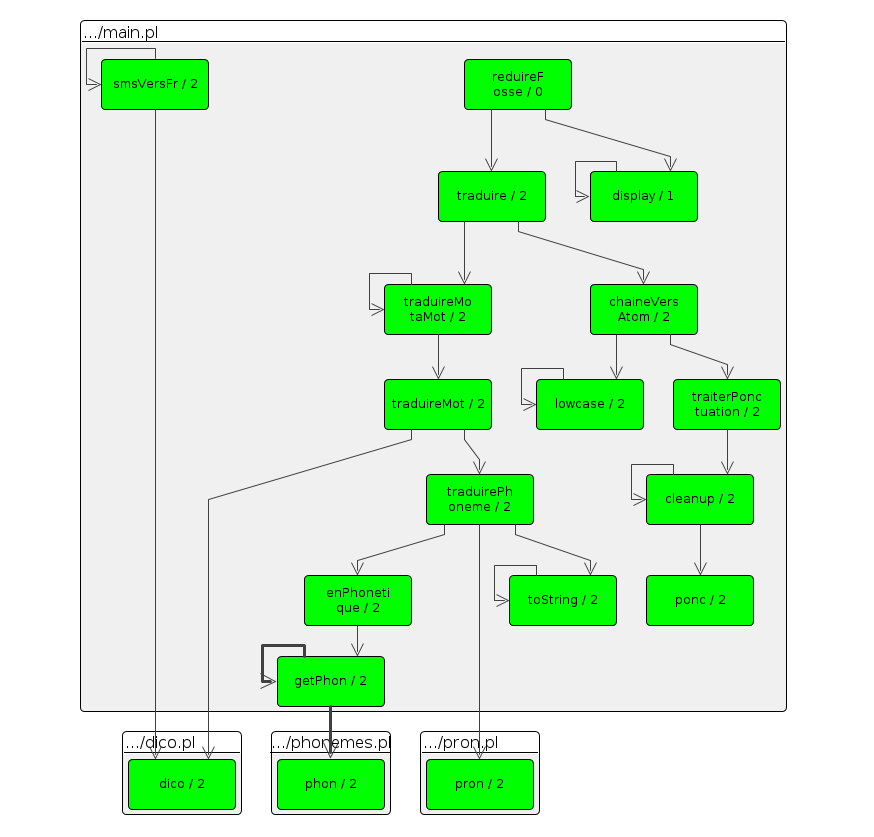
\includegraphics[scale=0.25]{mainpl.png}
	\end{figure}
\end{frame}

\begin{frame}{Conclusion}
	\begin{itemize}
		\item Il reste encore de nombreuse amélioration à apporter
		\item Le dictionnaire Français/phonétique contient de nombreuse mauvaise occurrence
		\item On pourrait explorer la piste des modèles de langue
		\item Enfin, on pourrait concevoir une GUI afin d'embarquer le logiciel sur smartphone
	\end{itemize}
\end{frame}

\end{document}